\documentclass[10pt]{beamer}

\usepackage{appendixnumberbeamer}
%
%\usepackage{lmodern}
%\usepackage{wrapfig}
\usepackage{tikz}
%\usetikzlibrary{positioning}
\usetikzlibrary{arrows,shapes}
\usepackage{amsmath,esint,esvect} % arrow for vector, maths and more
%\usepackage{datetime}
\usepackage{gensymb}%for degree symbol
%\usepackage{beamerthemesplit}
%\usepackage{graphicx} %trimed images
%\usepackage{pifont} %for dings
%
%\usepackage{import}
%\usepackage{cases}
\usepackage{booktabs} %beautiful tables
\usepackage{pgfplots}
\usepgfplotslibrary{dateplot}
%
\usepackage{siunitx} % SI notations
\sisetup{table-number-alignment=center, exponent-product=\cdot}




% Bibliography includes
\usepackage[backend=bibtex, citestyle=verbose-trad2,bibstyle=authortitle-icomp,sortcites=true,block=space,firstinits=true]{biblatex}
\addbibresource{2019_LM_Euroscipy.bib}
\usepackage{hyperref}

\usetheme[progressbar=frametitle]{metropolis}



    \setbeamertemplate{itemize subitem}{\color{orange}$\blacktriangleright$}

% --------------Math mode------------------
\renewcommand\mathfamilydefault{\rmdefault}
% -----------------------------------------

% ------ Images path ------------------
\newcommand{\figurespath}{./figures}

%% ---------- Editing the footer ------------
%\makeatother
%\setbeamertemplate{footline}
%{
%  \leavevmode%
%  \hbox{%
%  \begin{beamercolorbox}[wd=.6\paperwidth,ht=2.25ex,dp=1ex,center]{institute in head/foot}% 
%    \usebeamerfont{institute in head/foot}\insertshortinstitute
%  \end{beamercolorbox}%
%  \begin{beamercolorbox}[wd=.4\paperwidth,ht=2.25ex,dp=1ex,center]{date in head/foot}%
%    \usebeamerfont{date in head/foot}\insertshortdate\hspace*{2em}
%     \insertframenumber{} \hspace*{2ex}
%  \end{beamercolorbox}}%
%  \vskip0pt%
%}
%\makeatletter
%\setbeamertemplate{navigation symbols}{}
%% -----------------------------------------

% ------ Date definition ------------------
% \newdate{date}{04}{09}{2019}
% -----------------------------------------

% ----------New color----------------------
\definecolor{myblue}{RGB}{51,51,179}
\definecolor{beaubleu2}{cmyk}{1,0,0,0.71}
\definecolor{SchoolColor}{rgb}{0.6471, 0.1098, 0.1882} % Crimson
\definecolor{beaurouge}{HTML}{405684}
\definecolor{beaubleu}{HTML}{CC382C}
\definecolor{myyellow}{rgb}{0.99, 0.82, 0.35}
% -----------------------------------------

%% ---------Redifining foot cites-----------
\newrobustcmd*{\footlessfullcite}{\AtNextCite{\renewbibmacro{title}{}\renewbibmacro{in:}{}}\footfullcite}

%\renewbibmacro{in:}{\hspace{-5pt}}
%\AtEveryCitekey{\clearfield{pages}\clearfield{volume}\clearfield{url}
%\clearfield{doi}\clearfield{issn}}
%% -----------------------------------------

% ---------First page variables------------
\title{ToFu}
\subtitle{An open-source python/cython library for synthetic tomography diagnostics on tokamaks}
\author[Laura S. Mendoza] % (optional, for multiple authors)
{\textbf{Laura~S.~Mendoza}\inst{1}, \and Didier~Vezinet\inst{2}}
\institute[] % (optional)
{
	\inst{1}%
	INRIA Grand-Est,
	TONUS Team, Strasbourg, France\\
	
	\inst{2}%
	CEA,
	Cadarache, France
}
\date[\displaydate{date}] % (optional)
{\alert{Euroscipy 2019, Bilbao, Espa\~na}}
\subject{}


% -----------------------------------------

%%%%%%%%%%%%%%%%%%%%%%%%%%%%
\begin{document}

\newcommand{\gradx}{\nablax}
\newcommand{\vpar}{v_\parallel}
\newcommand{\xvec}{\mathbf{x}}
\newcommand{\nablax}{\nabla_{\!\xvec}}


% =================================
%\usebackgroundtemplate{
\includegraphics[height=\paperheight,width=\paperwidth]{figures/background.png}}%
\begin{frame}
    \titlepage
\end{frame} 
% =================================

% =================================
\begin{frame}{Table of contents}
  \setbeamertemplate{section in toc}[sections numbered]
  \tableofcontents[hideallsubsections]
\end{frame}
% =================================

\section{Context}

% =================================
\begin{frame}
\frametitle{Context: Energy generation}

	\begin{center}
		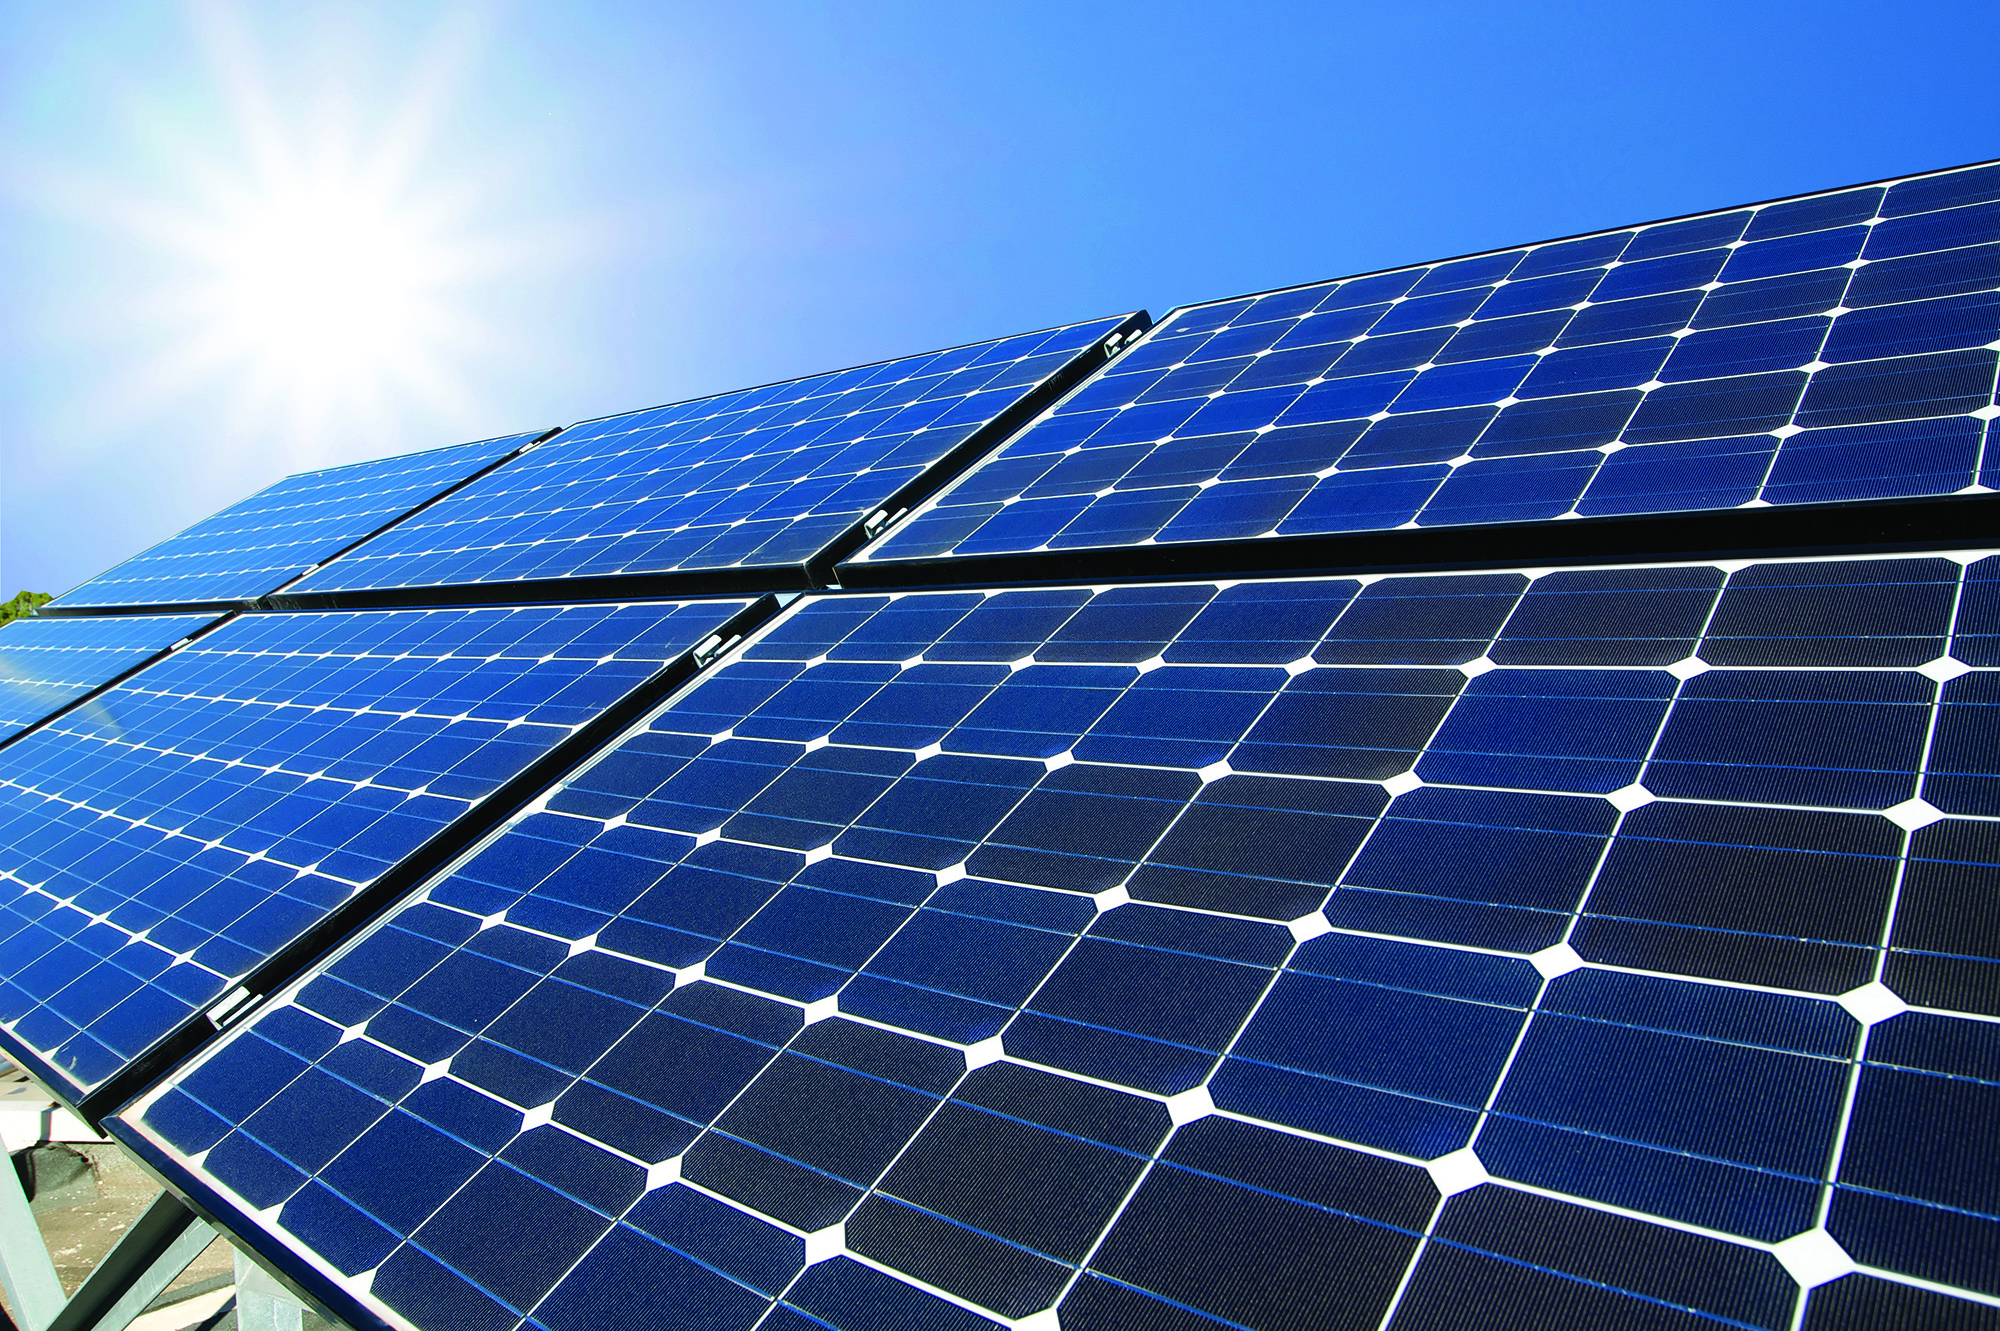
\includegraphics[height=2.2cm]{figures/solar-power.jpg}%
		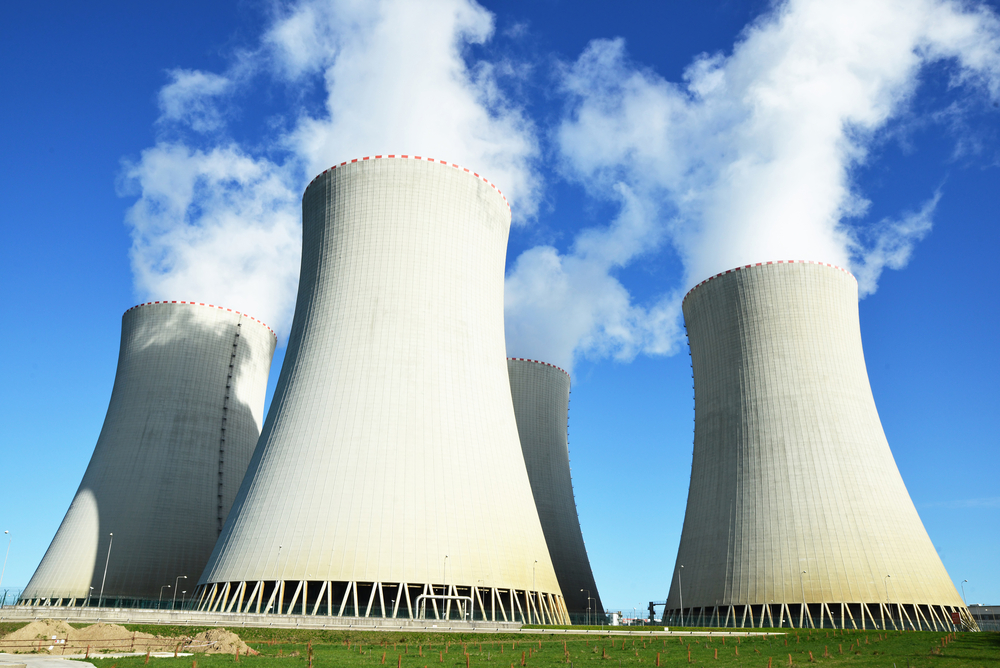
\includegraphics[height=2.2cm]{figures/nuclear-power.jpg}%
		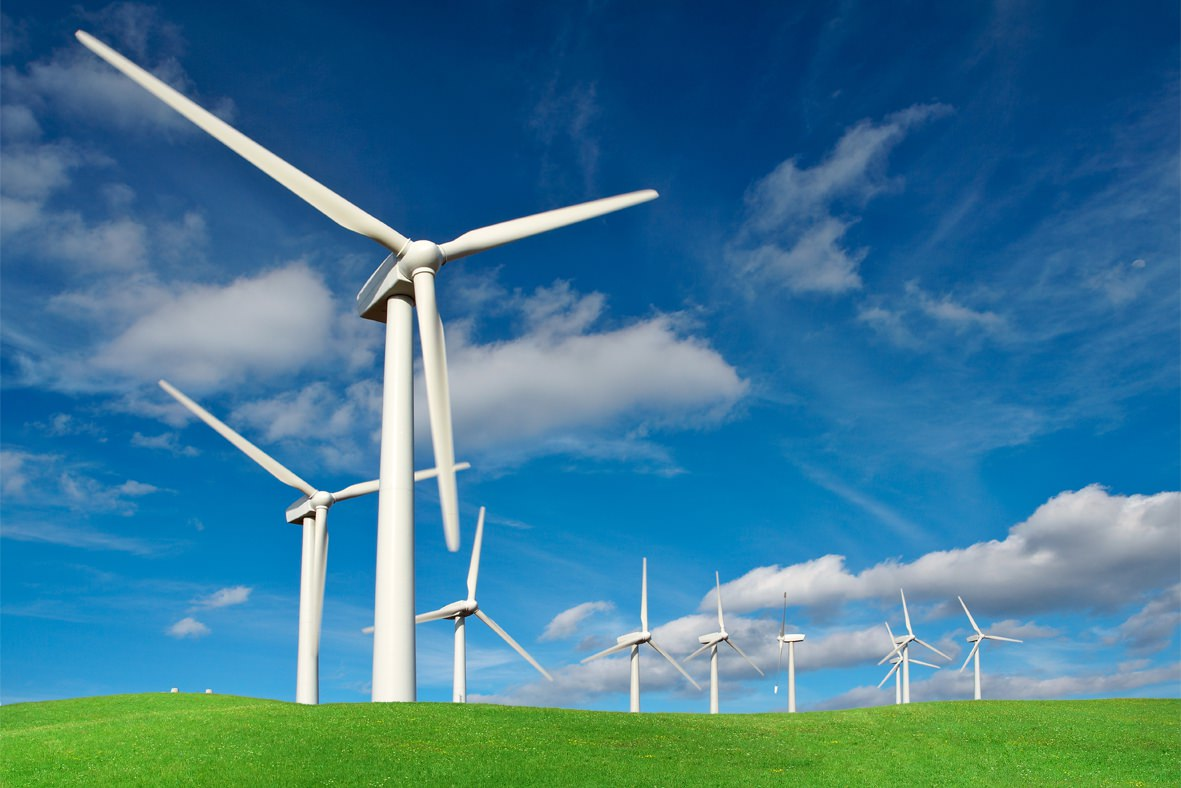
\includegraphics[height=2.2cm]{figures/wind-power.jpg}
	\end{center}

Current solutions present some drawbacks:
\begin{itemize}%[leftmargin=1em]
	\item Limited resources
	\item Production of carbon dioxide
	\item Radioactive waste
	\item Not too efficient
	\item Harmful to surrounding environment
\end{itemize}

\begin{itemize}%[leftmargin=1em]
\setbeamertemplate{itemize item}{$\Rightarrow$}
	\item \alert{Fusion}: cleaner, more reliable, more powerful energy source?
\end{itemize}

\end{frame}
% =================================



% =================================
\begin{frame}
\frametitle{Context: Controlled fusion and magnetic confinement}
    
\begin{columns}
    	\begin{column}{0.65\textwidth}
    	    	\begin{center}
		\textbf{D-T Fusion reaction\;\;\;}\vspace{0.3cm}
		%\includegraphics[width=3.5cm]{figures/DT_reaction3.png}
    		\resizebox{0.5\textwidth}{!}{% !TEX root = ../LM_defense.tex
% \begin{center}


\pgfdeclareradialshading{sphere}{\pgfpoint{0cm}{0cm}}% 
{rgb(0cm)=(1,1,1);
rgb(0.7cm)=(0.7,0.1,0); rgb(1cm)=(0.5,0.05,0); rgb(1.05cm)=(1,1,1)}

 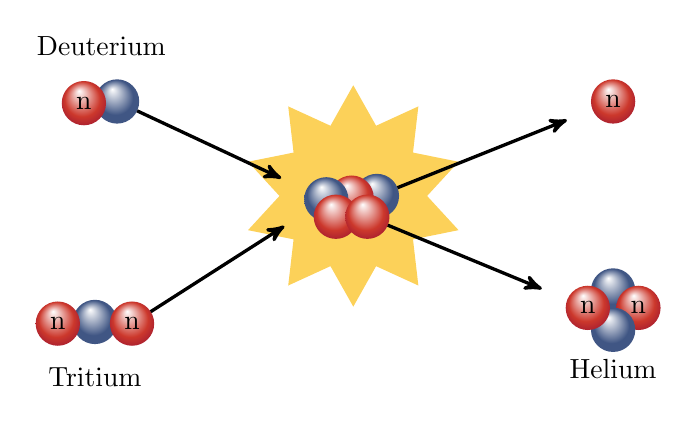
\begin{tikzpicture}[->,>=stealth',shorten >=10pt,auto,node distance=3cm,
 very thick, color=black]
 
 \pgfdeclareradialshading{redsphere}{\pgfpoint{-0.2cm}{0.5cm}}% 
{rgb(0cm)=(1,1,1);
color(0.7cm)=(beaurouge); color(1cm)=(beaurouge); rgb(1.05cm)=(1,1,1)}

 \pgfdeclareradialshading{greysphere}{\pgfpoint{-0.2cm}{0.5cm}}% 
{rgb(0cm)=(1,1,1);
color(0.7cm)=(beaubleu); color(1cm)=(SchoolColor); rgb(1.05cm)=(1,1,1)}


  \tikzset{plus/.style = {shape          = circle,
                                 ball color     = SchoolColor,
                                 text           = black,
                                 inner sep      = 0pt,
                                 outer sep      = 0pt,
                                 minimum size   = 16 pt,
				 shading = redsphere}}
				 
  \tikzset{neutron/.style   =  {shape          = circle,
                                 text           = black,
                                 inner sep      = 0pt,
                                 outer sep      = 0pt,
                                 minimum size   = 16 pt,
				 shading = greysphere}}
				 
  \tikzset{boom/.style =  {shape          = star,
				 star points = 10,
                                 fill    = myyellow,
                                 text           = black,
                                 inner sep      = 0pt,
                                 outer sep      = 0pt,
                                 minimum size   = 80 pt}}

  \node[plus] (Dplus) {};
  \node[neutron] (Dneutron) [below left of=Dplus,xshift=1.7cm,yshift=2.1cm]{n};

  \node[boom] (star)[right of=Dplus,yshift = -1.2cm] {};

  \node[plus] (Tplus2) [below of=Dplus,yshift=0.2cm,xshift=-8pt]{};
  \node[neutron] (Tneutron) [below right of=Tplus2,xshift=-1.65cm,yshift=2.1cm]{n};
  \node[neutron] (Tneutronbis) [below left of=Tplus2,xshift=1.65	cm,yshift=2.1cm]{n};

  \node[plus] (Rplus1) [right of=Dplus,yshift = -1.2cm,xshift=0.3cm] {};
  \node[neutron] (Rneutron1) [below left of=Rplus1,xshift=1.8cm,yshift=2.1cm]{};
  \node[plus] (Rplus2)  [below left of=Rneutron1,xshift=1.8cm,yshift=2.1cm]{};
  \node[neutron] (Rneutron2) [below right of=Rplus2,xshift=-2cm,yshift=1.9cm]{};
  \node[neutron] (Rneutron3) [right of=Rneutron2,xshift=-2.6 cm,yshift=0cm]{};


  \node[neutron] (Neutron) [right of=Rplus1,yshift=1.2cm]{n};

  \node[plus] (HePlus) [right of=Rplus1,yshift=-1.2cm]{};
  \node[neutron] (Heneu2) [below right of=HePlus,yshift=1.9cm,xshift=-1.8cm]{n};
  \node[plus] (HePlus2) [below of=HePlus,yshift=2.5cm]{};
  \node[neutron] (Heneu3) [below left of=HePlus,yshift=1.9cm,xshift=1.8cm]{n};
  
  \draw[->] (Dplus) to (Rplus2);
  \draw[->] (Tneutron) to (Rplus2);
  \draw[->] (Rplus1) to (Neutron);
  \draw[->] (Rneutron3) to (Heneu3);
  \node (texte1) [above of=Dplus,black,yshift=-2.3cm,xshift=-0.2cm] {Deuterium};
  \node(texte2)[below of=Tplus2,black,xshift=0cm,yshift=2.3cm] {Tritium};
  \node(texte3)[below of=HePlus,black,xshift=0cm,yshift=2cm] {Helium};

\end{tikzpicture}




}       
    		\end{center}
    		\vspace{-0.5cm}
		\begin{itemize}%[leftmargin=1em]
    			\item Gas $>$ 100 Million\degree K composed of positive ions and negative electrons: plasma
    			\item Confinement using electromagnetic fields
			\item Energy break-even point still not obtained: $Q_{\text{max}} = \dfrac{E_\text{output}}{E_\text{input}}  =0.67$
		\end{itemize}

    	\end{column}
    	
    	\begin{column}{0.35\textwidth}
	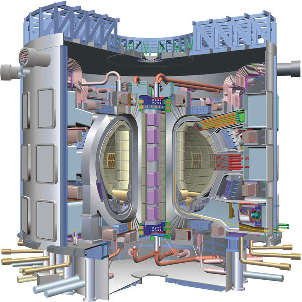
\includegraphics[width=1.\textwidth]{figures/ITER.pdf}
    	\end{column}
    	
\end{columns}

\begin{itemize}%[leftmargin=1em]
	\item Current reactors: different shapes, sizes, heating methods, confinement techniques, etc.
\end{itemize}
\vspace{-0.2cm}
\begin{itemize}%[leftmargin=1em]
\setbeamertemplate{itemize item}{$\Rightarrow$}
	\item \alert{Fusion codes:} complexity due to the number of parameters, geometry, model, etc.
\end{itemize}
\end{frame}
% =================================


\section{Tomography diagnostics}


% =================================
\begin{frame}
\frametitle{Tokamak diagnostics}
    
 \metroset{block=fill}
\begin{alertblock}{Diagnostics}
Set of instruments to measure for the understanding, control and optimization of the plasma performance.
\end{alertblock}

\begin{itemize}
\item \textbf{Magnetic} diagnostics: currents, plasma stored energy, plasma shape and position;

\item \textbf{Neutron} diagnostics (ie. cameras, spectrometers, etc.): fusion power;

\item Optical systems (\textbf{interferometers}): temperature and density profiles;

\item Bolometric systems (\textbf{tomography}): spatial distribution of radiated power;

\item \textbf{Spectroscopic}: X-ray wavelength range, impurity species and density, input particle flux, ion temperature, helium density, fueling ratio, plasma rotation, and current density.

%\item Microwave diagnostics probe the main plasma and the plasma in the divertor region in order to measure plasma position.

\end{itemize}

\end{frame}
% =================================


% =================================
\begin{frame}
\frametitle{Tomography diagnostics - numerical context}
    \vspace{-0.75cm}

    $$M_i(t) = \iiint\limits_{V_i} \vv{\varepsilon(x,t)}\cdot\vv{n} \,\Omega_i \;{d}V$$
    \vspace{-0.75cm}
\begin{columns}
    	\begin{column}{0.325\textwidth}
    	
    	%\def\svgwidth{\linewidth}
    	%\import{figures/}{detectors.pdf_tex}
    	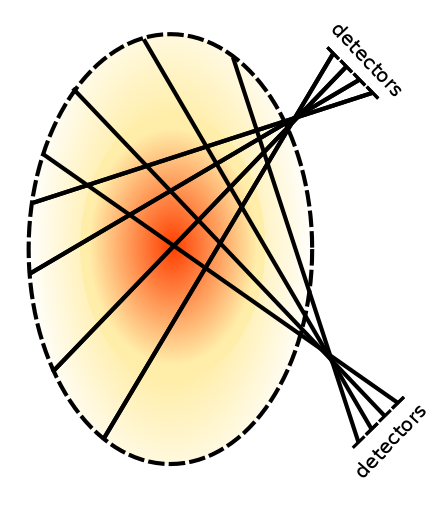
\includegraphics[width=\linewidth]{figures/detectors2.png}

    	\end{column}

   	\begin{column}{0.675\textwidth}
   	\begin{center}
   	
   	%DIRECT PROBLEM
   	\begin{block}{}
	\begin{itemize}
	\item \textcolor{myblue}{\textbf{Direct problem} (synthetic diagnostic):\\
	}
	\end{itemize}
	\end{block}
   		%\textbf{Direct problem} (synthetic diagnostic):\\
Simulated emissivity $\longrightarrow$ integrated measurements\\

	%INVERSE PROBLEM
   	\begin{block}{}
	\begin{itemize}
	\item \textcolor{myblue}{\textbf{Inverse problem} (tomography):\\
	}
	\end{itemize}
	\end{block}
   		%\textbf{Direct problem} (synthetic diagnostic):\\
Integrated measurements $\longrightarrow$ Reconstructed emissivity \\

   	\end{center}
	
   	\end{column}
%    	
\end{columns}


\end{frame}
% =================================




% =================================
\begin{frame}
\frametitle{Tomography diagnostics - numerical context}

    $$M_i(t) = \iiint\limits_{V_i} \vv{\varepsilon(x,t)}\cdot\vv{n} \,\Omega_i \;{d}V$$
    \vspace{-1cm}
\begin{columns}
    	\begin{column}{0.325\textwidth}
    	
    	%\def\svgwidth{\linewidth}
    	%\import{figures/}{detectors.pdf_tex}
    	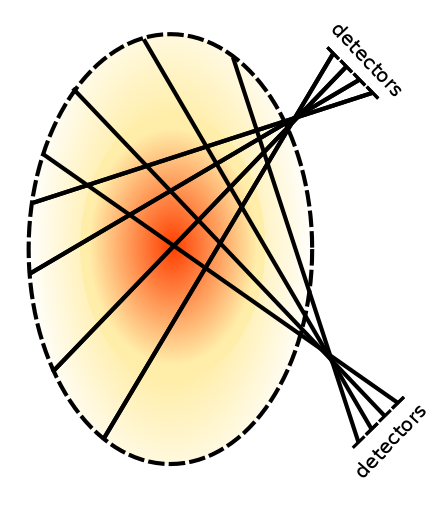
\includegraphics[width=\linewidth]{figures/detectors2.png}

    	\end{column}

   	\begin{column}{0.675\textwidth}
   	\begin{center}
   	
   	%DIRECT PROBLEM
   	\begin{block}{}
	\begin{itemize}
	\item \textcolor{myblue}{\textbf{Direct problem} (synthetic diagnostic):\\
	}
	\end{itemize}
	\end{block}
   		%\textbf{Direct problem} (synthetic diagnostic):\\
Simulated emissivity $\longrightarrow$ measurements\\
	\alert{Spatial integration}
    \vspace{-0.5cm}

	%INVERSE PROBLEM
   	\begin{block}{}
	\begin{itemize}
	\item \textcolor{myblue}{\textbf{Inverse problem} (tomography):\\
	}
	\end{itemize}
	\end{block}
   		%\textbf{Direct problem} (synthetic diagnostic):\\
Integrated measurements $\longrightarrow$ Reconstructed emissivity \\
	 \alert{Mesh and basis functions construction, spatial integration, data filtering, inversion routines, etc.}
   	
   	\end{center}
	
   	\end{column}
%    	
\end{columns}

\pause
\vspace{-0.5cm}
\begin{block}{}
\begin{center}
Tomography very sensitive to errors, noise and bias\\
$\longrightarrow$  \alert{Reputation for low reproducibility / reliability }
\end{center}
	\end{block}
\end{frame}
% =================================



\section{The ToFu code}


% =================================
\begin{frame}
\frametitle{Motvation: ``current" state}

	In the fusion community, codes for synthetic diagnostic are developed:
	\begin{itemize}
		\item  by physicists (with little to no programming experience),
		\item  in Matlab,
		\item  from scratch,
		\item  in local/private 
	\end{itemize}

... which means
\begin{itemize}
		\item  repetition of work: lost time, man-power, etc;
		\item  no traceability,
		\item  results impossible to reproduce,
		\item  no standardization of diagnostics
	\end{itemize}
	
\end{frame}
% =================================


% =================================
\begin{frame}
\frametitle{A code for Tomography for Fusion}
\textbf{Develop a common tool:}
\begin{columns}
\begin{column}{0.65\textwidth}
	\begin{itemize}
	\item Accessible to everyone (open-source)
	\item Generic (geometry independent)
	\item Portable (developed in Python)
	\item Optimized (reliability and performance)
	\item Documented online
	\item Continuous integration
	\end{itemize}
\end{column}
\begin{column}{0.35\textwidth}
\vspace{-1cm}
\begin{center}
    	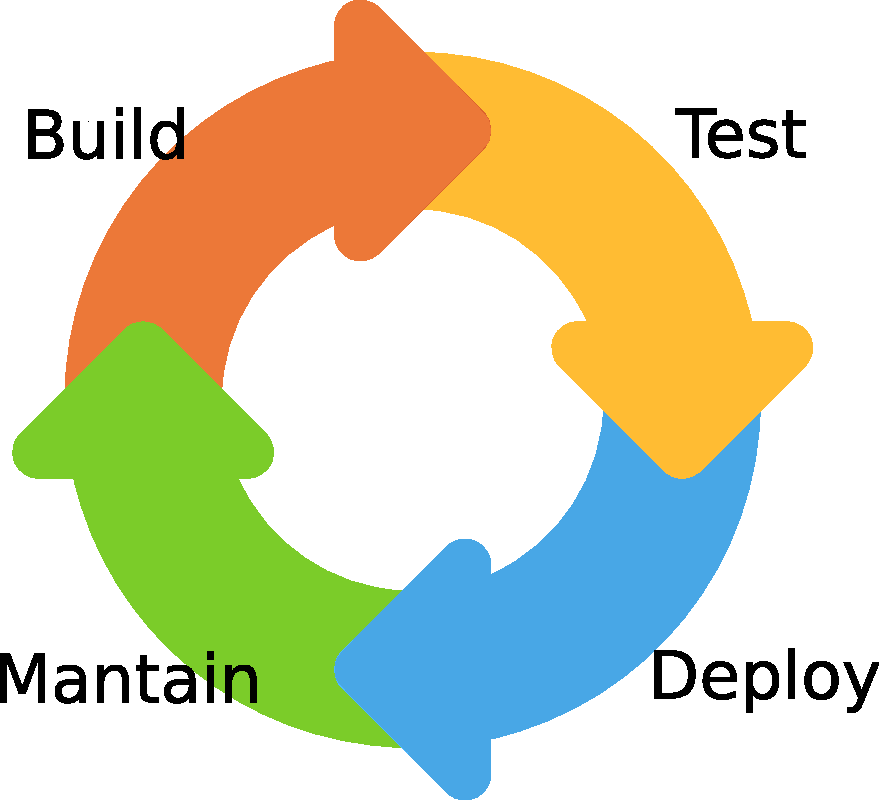
\includegraphics[width=0.8\linewidth]{figures/ci.pdf}
\end{center}
\end{column}
\end{columns}

\begin{block}{}
	\begin{center}
	\textbf{For tomography diagnostics:\\ } The \textcolor{SchoolColor}{\textbf{To}mography for \textbf{Fu}sion} code (\textcolor{SchoolColor}{\textbf{ToFu}\footnote{repository: \url{https://github.com/ToFuProject/tofu}}\footnote{documentation: \url{https://tofuproject.github.io/tofu/index.html} }\footcite{didier2016}})
	\end{center}
\vspace{-5mm} 
\end{block}
	
\end{frame}
% =================================

% =================================
\begin{frame}
\frametitle{More about Tofu}

\begin{columns}
\begin{column}{0.65\textwidth}
\begin{itemize}
	\item Created in 2014
	\item Open Source:\textbf{ MIT license}
	\item Python 2.7 and \textbf{Python} 3 + \textbf{Cython}
	\item Continuous integration: \textbf{Travis} CI
	\item \textbf{conda}, \textbf{pip}
	\item Two (main) developers:
	\begin{itemize}
		\item Didier Vezinet (creator, PhD in Physics)
		\item Laura S. Mendoza (since June 2018, PhD in Applied Mathematics)
	\end{itemize}
	\item Contributors:
	\begin{itemize}
		\item Jorge Morales (PhD in Physics)
		\item Florian Le Bourdais
		\item Arpan Khandelwal (intern)
	\end{itemize}
\end{itemize}
\end{column}
\begin{column}{0.35\textwidth}
\begin{center}
    	
\includegraphics[width=\textwidth]{figures/qr-code.png}
\end{center}
\end{column}
\end{columns}
\begin{center}
    	
\includegraphics[width=\textwidth]{figures/badges.png}
\end{center}

\end{frame}
% =================================

% Tofu peut:
%  Modeliser geom simplifiée
%  Modeliser geom 3D d'une camera 1D
%  Modeliser geom 3D d'une camera 2D
%  Handle basics of Reflexions
%  Calculer signal synthetic
% and next : meshing and basis functions, tomographic inversion

% =================================

% =================================
\begin{frame}
\frametitle{What ToFu can do: modeling of simplified geometry}
	
\end{frame}
% =================================

% =================================
\begin{frame}
\frametitle{What ToFu can do: 3D modeling of a 1D camera}
	
\end{frame}
% =================================

% =================================
\begin{frame}
\frametitle{What ToFu can do: 3D modeling of a 2D camera}
	
\end{frame}
% =================================

% =================================
\begin{frame}
\frametitle{What ToFu can do: handle basic reflexions}
	
\end{frame}
% =================================

% =================================
\begin{frame}
\frametitle{What ToFu can do: computing synthetic signals}
	
\end{frame}
% =================================

% =================================
\begin{frame}
\frametitle{What ToFu can do}
ToFu can:
\begin{itemize}
	\item Modeling of simplified geometry
	\item 3D modeling of a 1D camera
	\item 3D modeling of a 2D camera
	\item Handle basic reflexions
	\item Computing synthetic signals
	\item ...and soon:
		\begin{itemize}
			\item meshing and basis functions
			\item tomographic inversion
			\item dust particle trajectory tracking
			\item faster Matplotlib + PyQtGraph visualization
			\item magnetic field line tracing
			\item data visualization and statistical tools (pandas)
		\end{itemize}
\end{itemize}
\end{frame}
% =================================
\section{Demo}

% =================================
{\setbeamercolor{palette primary}{fg=black, bg=yellow}
\begin{frame}[standout]
  Demo
\end{frame}
}
% =================================

% =================================
\begin{frame}
\frametitle{Tofu's structure}

\begin{center}
    	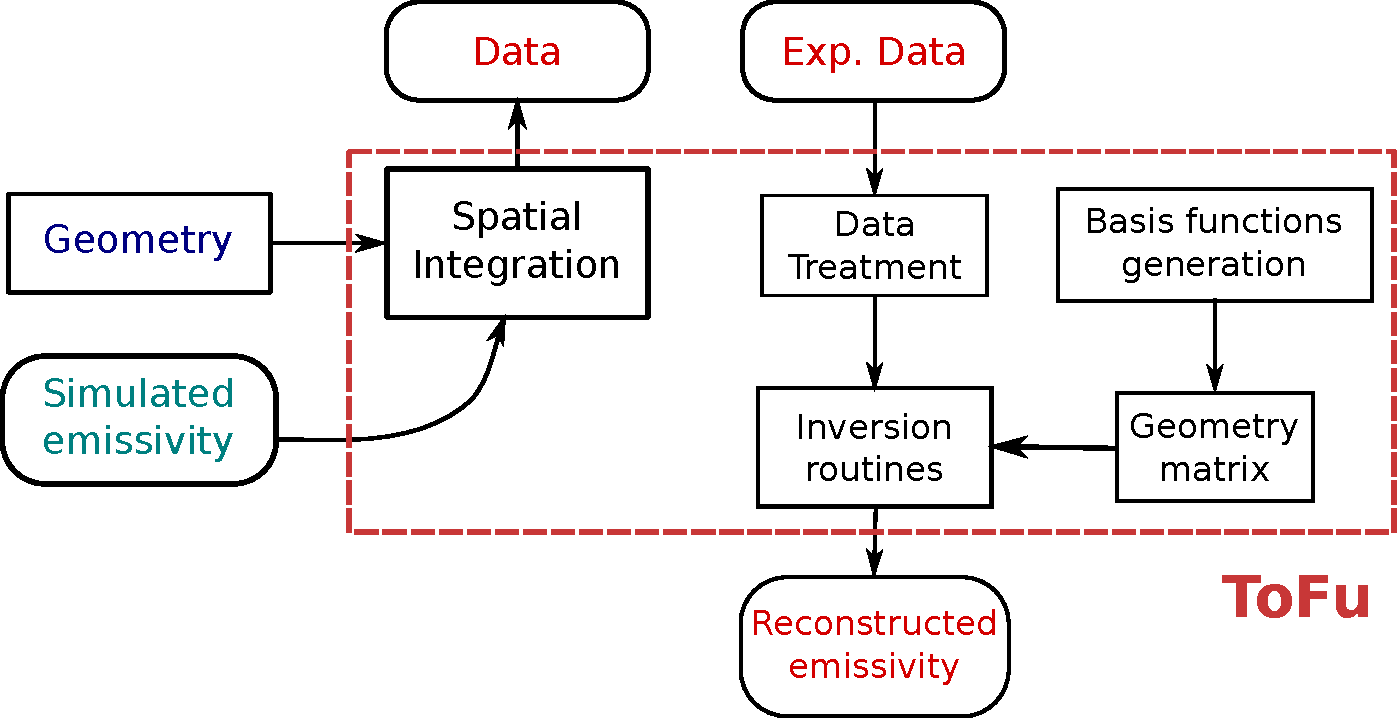
\includegraphics[width=0.8\linewidth]{figures/tofu.pdf}
\end{center}
	
\end{frame}
% =================================

\section{Optimization of the code}

% =================================
\begin{frame}
\frametitle{Geometry reconstruction: ray-tracing techniques}

	To reconstruct emissivity we need to take account:
	\begin{itemize}
	\item Up to hundreds of structural elements in vessel
	\item Scale of the vessel:
	$10^4$ bigger than smaller structural detail
	\setbeamertemplate{itemize item}{$\Rightarrow$}

	\item Geometry defined with minimal data polygon $(R,Z)$\\ extruded along $\varphi$
	\item Symmetry of vessel along $\varphi$
	
	\end{itemize}
	
	\vspace{0.5cm}
	\begin{center}
		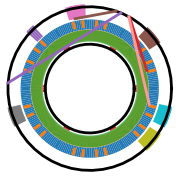
\includegraphics[height=2.3cm]{figures/confB3_wp_view2.png}%
		~
		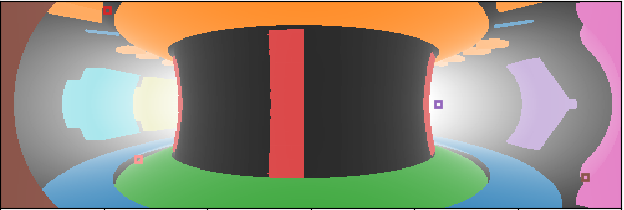
\includegraphics[height=2.3cm]{figures/confB3_wp_view1.png}%
		~
		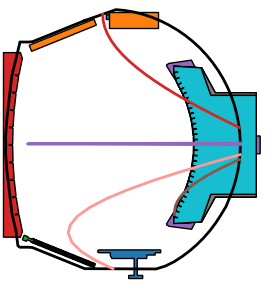
\includegraphics[height=2.3cm]{figures/confB3_wp_view3.png}%
	\end{center}
	
\end{frame}
% =================================



% =================================
\begin{frame}
\frametitle{Optimization of ray-tracing algorithm}

\begin{columns}
\begin{column}{0.65\textwidth}
	\begin{itemize}
	\item Description of geometry:
	\begin{itemize}
		\item Vessel and structures:  set of 2D polygon $\mathcal{P}_j = \cup_{i=1}^n \overline{{\rm A}_i{\rm B}_i}$
		\item Extruded along $[\varphi_{min}, \varphi_{max}]$
		\item Detectors defined as set of rays (of origin $D$ and direction $u$)
		\item[{$\Rightarrow$}] Light memory-wise
	\end{itemize}
	\item[{$\Rightarrow$}] Equivalent to: set of truncated cones (frustums) of generatrix $A_iB_i$
	
	\end{itemize}
\end{column}
\begin{column}{0.35\textwidth}
\begin{center}
    	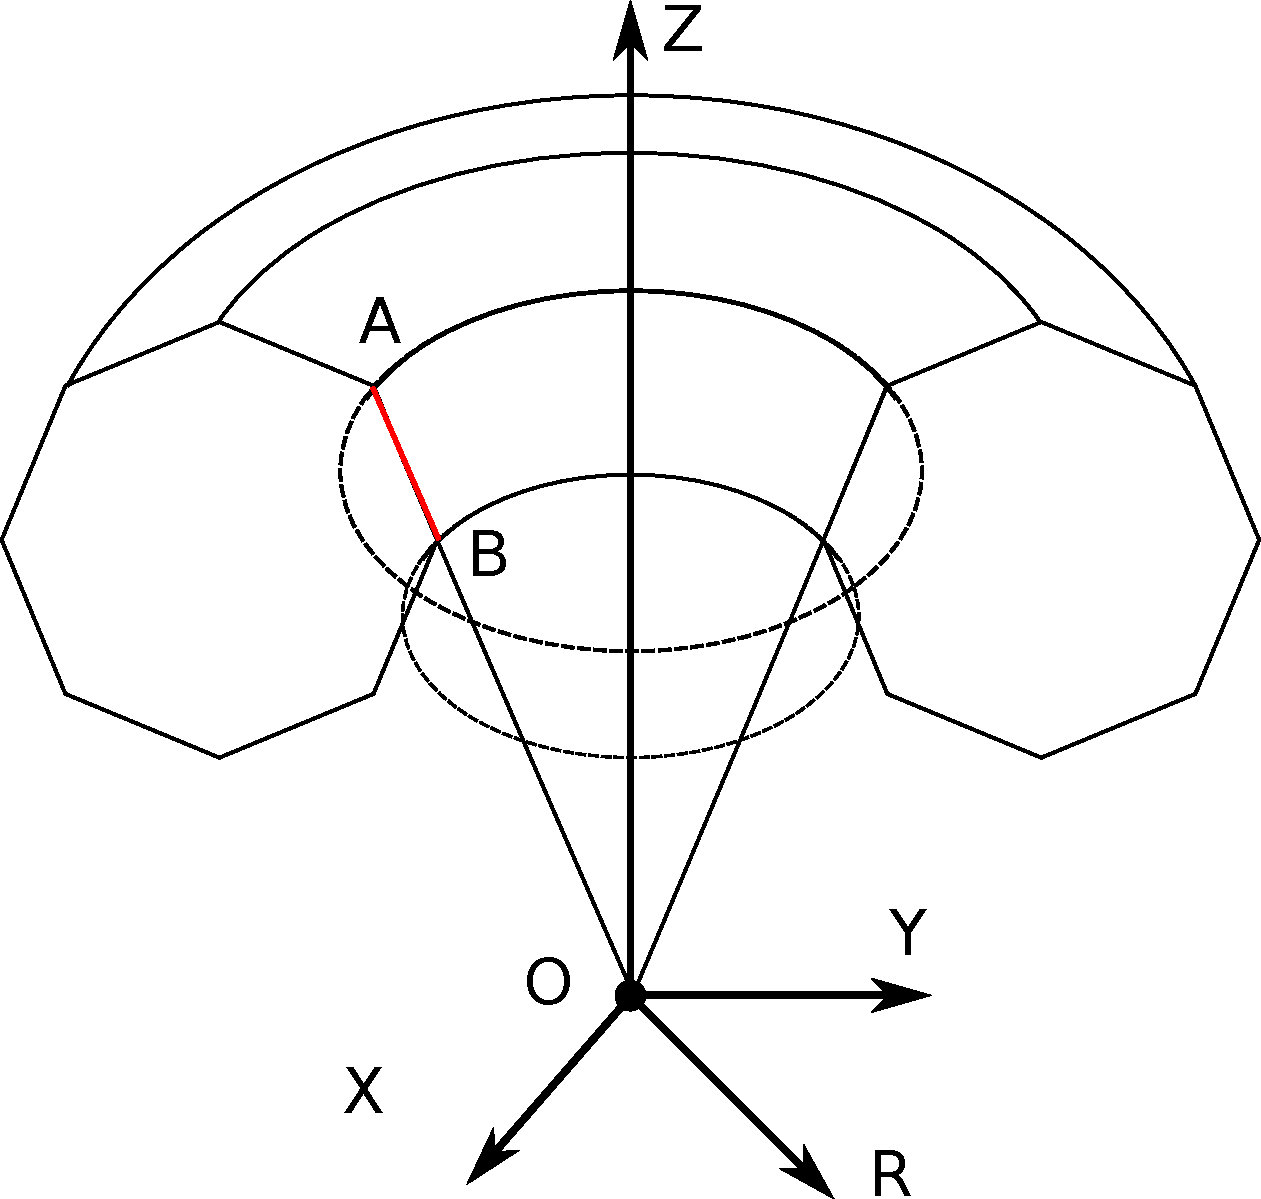
\includegraphics[width=\linewidth]{figures/tore_cones1.pdf}
\end{center}
\end{column}
\end{columns}

\vspace{0.3cm}
\begin{alertblock}{Ray-tracing algorithm on fusion device $\longrightarrow$ Computation of cone-Ray intersection}
\end{alertblock}

$$
\hspace{-3cm}
\exists (q,k) \in [0;1]\times [0;\infty[, \;
\left\{\begin{array}{ll}
R-R_A = q(R_B-R_A)\\
Z-Z_A = q(Z_B-Z_A)\\
DM = k u
\end{array}\right.
$$
	
\end{frame}
% =================================


% =================================
\begin{frame}
\frametitle{Optimization of ray-tracing algorithm}


Cone-Ray intersection algorithm:
	\begin{itemize}
	\item Main steps:
	\begin{itemize}
		\item Test if intersection with bounding-box
		\item Computation of special cases of segment $AB$
		\item Computation of special cases of ray directional vector
		\item General case: solution of a quadratic equation
	\end{itemize}
	\item Pre-computation of geometry-independent variables
	\item Core functions written in \textbf{Cython}
	\item Parallelization over ray-loop (\textbf{prange} loops)
	\end{itemize}

% TODO : moins de texte au dessus
\begin{table}[h] % just use this specifier if really needed.
    \centering
    \label{tab:LOS_init_sirrah}
    % Visionner le code LaTeX du paragraphe 0
	\sisetup{round-mode=places}
     \begin{tabular}{@{}l*{4}{S[table-format=1.2e-1,scientific-notation=true]}@{}}
       \toprule
       \textbf{Nb LOS} &  {$10^3$} & {$10^4$} & {$10^5$} & {$10^6$}\\
       \midrule
       original       & 32.569 & 310.23 & 3202.38 & 31723.827 $(~8$h$48)$\\
       optimized   & 0.0258 & 0.2720 & 2.73581 & 26.589564 $(<30$s$)$\\
       32 threads & 0.0136 & 0.0466 & 0.3640 & 2.9188 \\
       \bottomrule
     \end{tabular}
\end{table}

	
\end{frame}
% =================================


% =================================
\begin{frame}
\frametitle{Tofu's structure}

\begin{center}
    	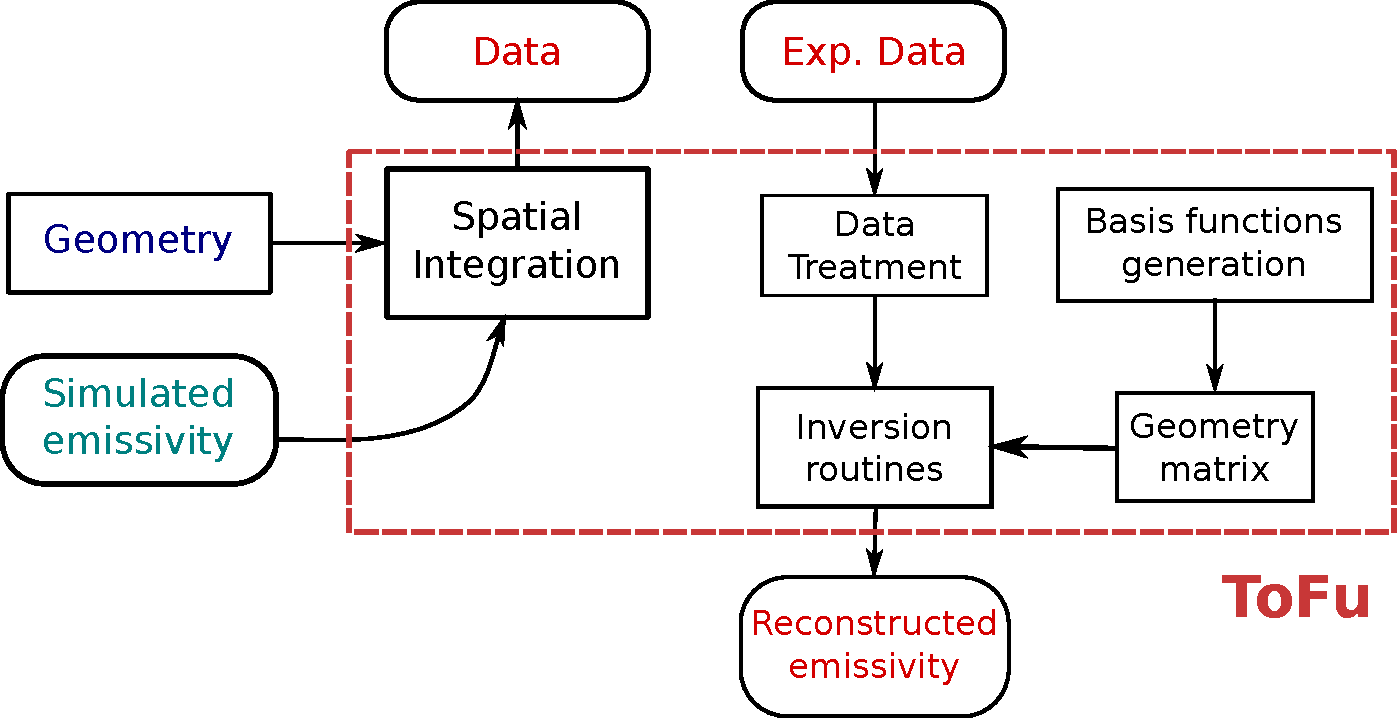
\includegraphics[width=0.8\linewidth]{figures/tofu.pdf}
\end{center}
	
\end{frame}
% =================================



% =================================
\begin{frame}
\frametitle{Optimization of spatial integration routines}

For the integration along a LOS:
% rajouter equation et redire que fonction definie par utilisateur
	\begin{itemize}
	\item Sample (discretization) of a 3D ray:
		\begin{itemize}
		\item Different quadrature rules: midpoint, simpson, romberg
		\item Resolution given by user
		\item Possible to define a sub-domain of discretization
		\end{itemize}
	\item Integration of a python function \textbf{func} defined by user by:
		\begin{itemize}
		\item \textbf{numpy}.sum
		\item Cython based sum
		\item \textbf{Scipy}.integrate.simps
		\item \textbf{Scipy}.integrate.romb
		\end{itemize}
	\item Optional optimizations:
		\begin{itemize}
		\item calls to \textbf{func}: avoid Cython-Python conversion, user-defined
		\item memory: fine resolutions, high number of LOS
		\item hybrid: compromise
		\end{itemize}
	\end{itemize}
	
\end{frame}
% =================================


%% =================================
%\begin{frame}
%\frametitle{Optimization of spatial integration routines}
%  \begin{figure}
%    \begin{tikzpicture}
%      \begin{axis}[
%        mbarplot,
%        xlabel={Number of Lines of Sight},
%        ylabel={Execution time},
%        width=0.9\textwidth,
%        height=6cm,
%        xticklabels={$0$,,$10$,,$10^2$, ,$10^3$,,$10^4$}]
%      ]
%
%      \addplot plot coordinates {(1, 0.46) (2, 2.24) (3, 18.1) };
%      \addplot plot coordinates {(1, 18) (2, 24) (3, 23.5) (4, 13.2)};
%      \addplot plot coordinates {(1, 0.2) (2, 0.53) (3, 4.32) (4, 40)};
%      \addplot plot coordinates {(1, 0.08) (2, 0.44) (3, 4.4) (4, 40)};
%
%      \legend{ref, mem, calls, hybd}
%
%      \end{axis}
%    \end{tikzpicture}
%  \end{figure}
%  \vspace{-0.2cm}
%    \begin{itemize}
%  \item Space resolution: $10^{-3}$
%  \item Number of time steps: $10^3$
%  \item Integration method: \textbf{sum} (Cython or numpy) on midpoint
%  \end{itemize}
%  \end{frame}
%  
%
%% =================================



% =================================
\begin{frame}
\frametitle{Optimization of spatial integration routines}

\begin{table}[h] % just use this specifier if really needed.
    \centering
    \label{tab:LOS_init_sirrah}
    % Visionner le code LaTeX du paragraphe 0
	\sisetup{round-mode=places}
     \begin{tabular}{@{}lllll@{}}
       \toprule
       \textbf{LOS} &  {$10$} & {$10^2$} & {$10^3$} & {$10^4$} \\% & {$10^5$}\\
       \midrule
       original       & 0.46 & 2.24 & 18.1 & x \\%& x \\
       memory   & 0.9 & 8.9 & 96 & 945 (6Gb)\\
       calls   & 0.207 & 0.53 & 4.32 & x \\
       hybrid & 0.08 & 0.44 & 4.2 & 40.3 (32Gb) \\%& 612 (32Gb)\\
       \bottomrule
     \end{tabular}
\end{table}

  \vspace{-0.2cm}
    \begin{itemize}
  \item Space resolution: $10^{-3}$
  \item Number of time steps: $10^3$
  \item Integration method: \textbf{sum} (Cython or numpy) on midpoint
  \end{itemize}
  \end{frame}
% =================================


\section{What's next}


% =================================
\begin{frame}
\frametitle{Tofu's structure}

\begin{center}
    	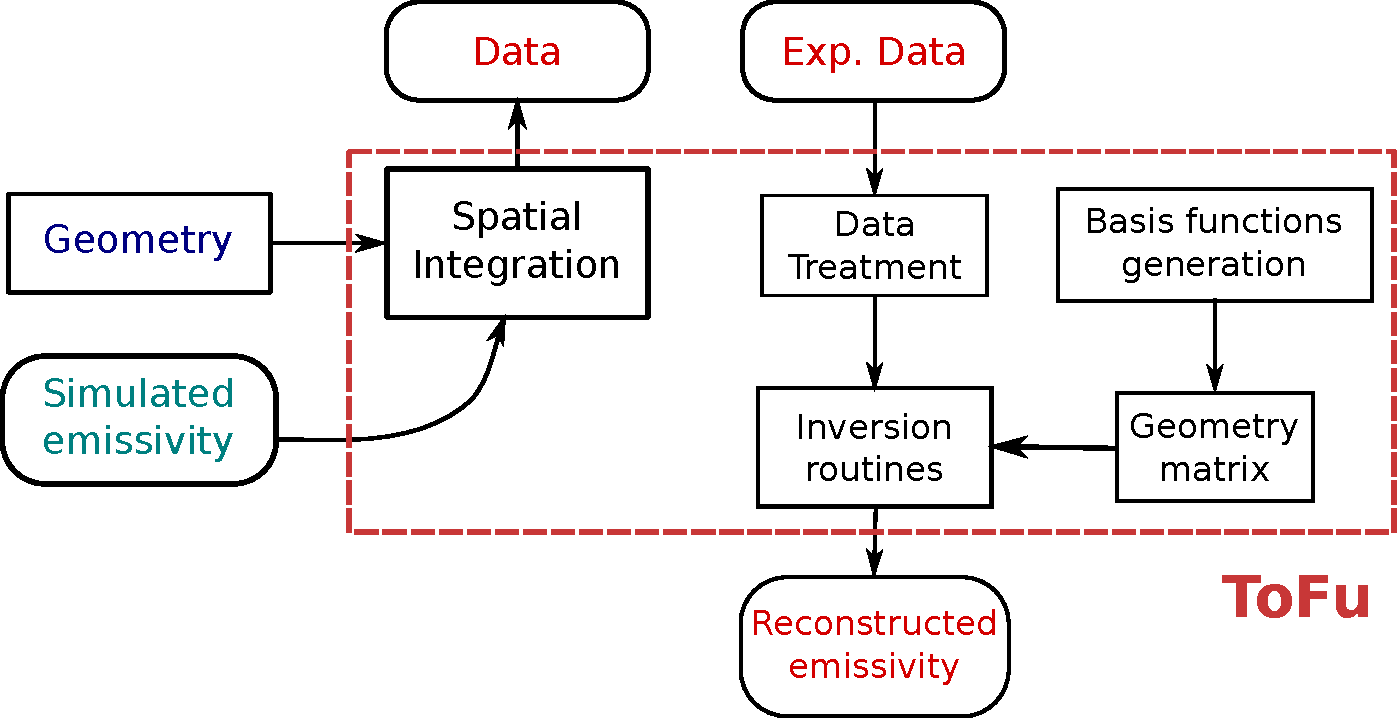
\includegraphics[width=0.8\linewidth]{figures/tofu.pdf}
\end{center}
	
\end{frame}
% =================================

%
%% =================================
%\begin{frame}
%\frametitle{Optimization of ray-tracing algorithm}
%
%
%$$
%\hspace{-3cm}
%\exists (q,k) \in [0;1]\times [0;\infty[, \;
%\left\{\begin{array}{ll}
%R-R_A = q(R_B-R_A)\\
%Z-Z_A = q(Z_B-Z_A)\\
%DM = k u
%\end{array}\right.
%$$
%\vspace{-0.5cm}
%\begin{columns}
%\begin{column}{0.65\textwidth}
%	\begin{itemize}
%	\item Vessel and structures defined as polygons
%	\item Algorithm based on \textbf{cone-ray intersection}
%	\item Core functions written in \textbf{cython}
%	\item Parallelization using \textbf{OpenMP}
%	\end{itemize}
%\end{column}
%\begin{column}{0.35\textwidth}
%\vspace{-1cm}
%\begin{center}
%    	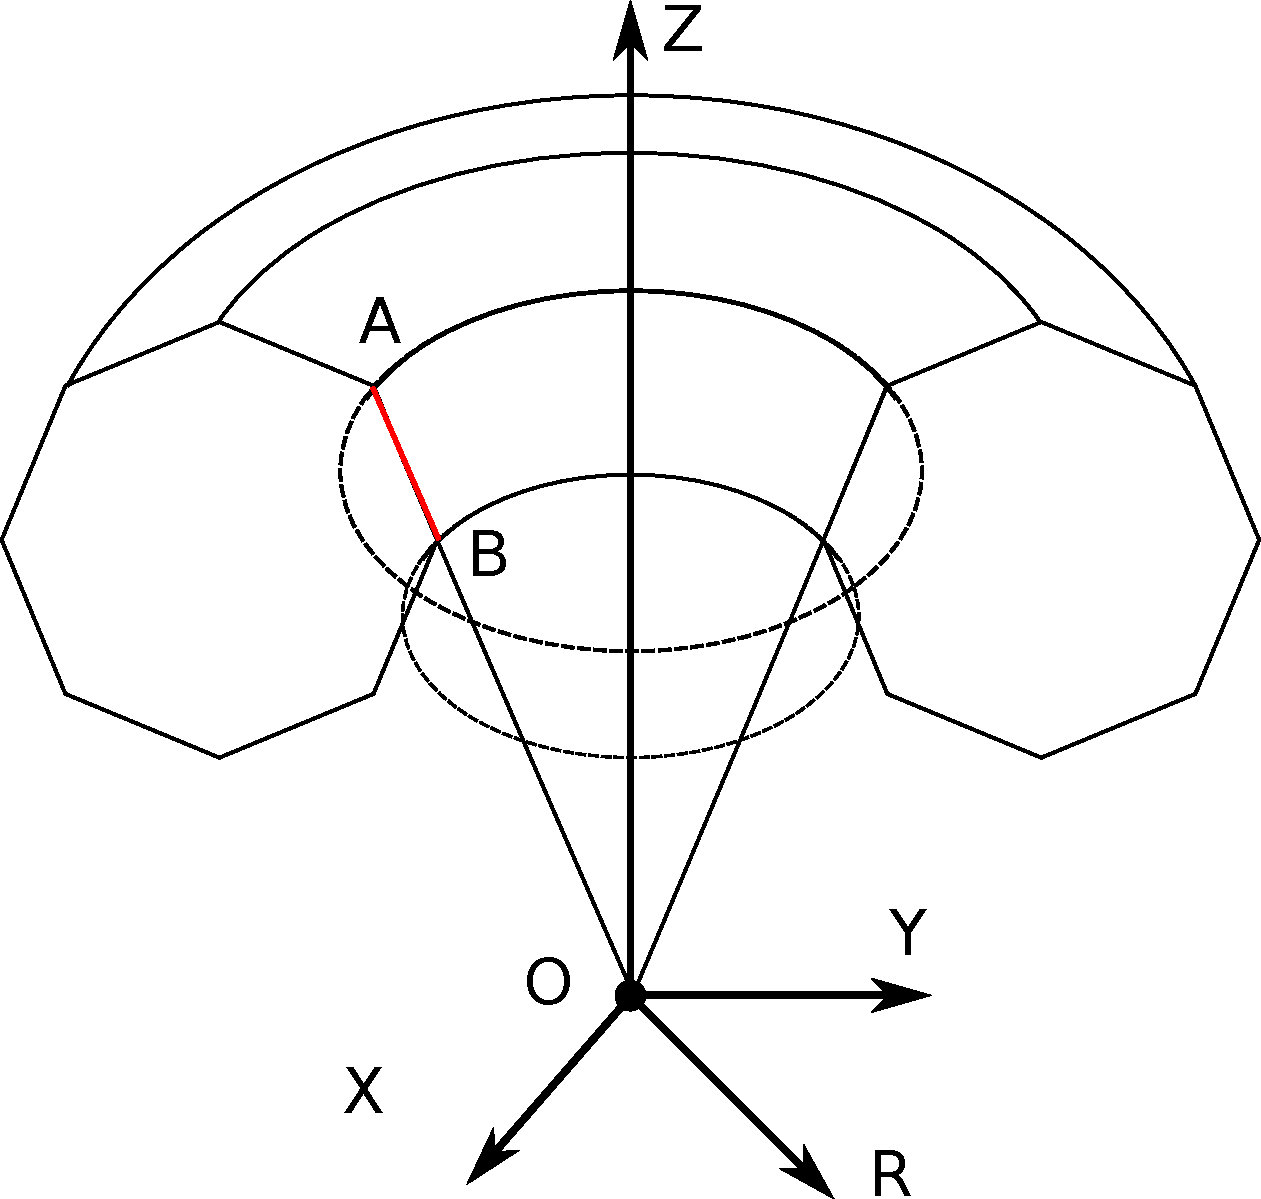
\includegraphics[width=\linewidth]{figures/tore_cones1.pdf}
%\end{center}
%\end{column}
%\end{columns}
%
%\begin{table}[h] % just use this specifier if really needed.
%    \centering
%    \label{tab:LOS_init_sirrah}
%    % Visionner le code LaTeX du paragraphe 0
%	\sisetup{round-mode=places}
%     \begin{tabular}{@{}l*{4}{S[table-format=1.2e-1,scientific-notation=true]}@{}}
%       \toprule
%       \textbf{Nb LOS} &  {$10^3$} & {$10^4$} & {$10^5$} & {$10^6$}\\
%       \midrule
%       original       & 32.569 & 310.23 & 3202.38 & 31723.827 $(~8$h$48)$\\
%       optimized   & 0.0258 & 0.2720 & 2.73581 & 26.589564 $(<30$s$)$\\
%       32 threads & 0.0136 & 0.0466 & 0.3640 & 2.9188 \\
%       \bottomrule
%     \end{tabular}
%\end{table}
%
%	
%\end{frame}
%% =================================





% =================================
\begin{frame}
\frametitle{On geometry discretization: meshing}


\begin{columns}
\begin{column}{0.6\textwidth}
Several options for poloidal cut meshing:

\begin{itemize}
	\item Cartesian mesh
	\item Polar mesh
	\item Adaptive polar mesh
	\item Hexagonal mesh
	\item Triangular mesh
\end{itemize}

\end{column}
\begin{column}{0.4\textwidth}

For basis functions:

\begin{itemize}
	\item Lagrange polynomials
	\item B-splines
	\item NURBS
	\item Box-splines
\end{itemize}
\end{column}
\end{columns}



\begin{center}
    	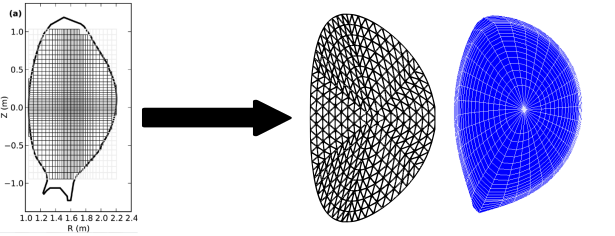
\includegraphics[width=0.85\linewidth]{figures/meshes.png}
\end{center}
\vspace{-0.5cm}
\end{frame}
% =================================




% =================================
\begin{frame}
\frametitle{Tofu's main algorithms}


\begin{columns}
\begin{column}{0.6\textwidth}
Visualization and geometrical tools:
	\begin{itemize}
	\item Ray-tracing algorithm
	\item Distance 3D objects and rays
	\item Vignetting: 3D polygon - Ray% intersection
	\item Solid angles computation (reflexions)
	\end{itemize}
\end{column}
\begin{column}{0.4\textwidth}

\begin{center}
    	\hspace{-0.5cm}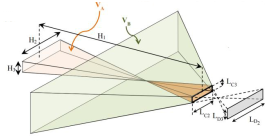
\includegraphics[width=\linewidth]{figures/cones.png}
\end{center}
\end{column}
\end{columns}

\vspace{0.2cm}
For direct and inverse problem:
\begin{itemize}
	\item Basis functions
	\item Discretization: Geometry, Lines, Volumes
	\item Spatial integration
	\item Regularization-inversion routines (Bayesian, non linear, etc.)
	\item Filtering
	\end{itemize}
%\begin{center}
%    	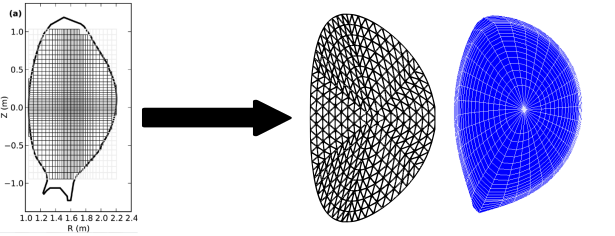
\includegraphics[width=0.6\linewidth]{figures/meshes.png}
%\end{center}	
\end{frame}
% =================================

% =================================
\begin{frame}
\centering
\Huge{Thank you for your attention!}
%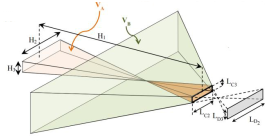
\includegraphics[width=\linewidth]{figures/cones.png}
\end{frame}
% =================================


% =================================
\subsection*{Splines interpolation}
\begin{frame}
	\frametitle{B(asis)-Splines basis*}

	B-Splines of degree $d$ are defined by the \textbf{recursion} formula: 

	\begin{equation}
	B_j^{d+1}(x)= \dfrac{x - x_j}{x_{j+d}-x_j} B_j^d(x)+ \dfrac{x_{j+1} - x}{x_{j+d+1} - x_{j+1}} B_{j+1}^d (x)
	\end{equation}

	Some important properties about B-splines:

	\begin{itemize}
		\item Piece-wise polynomials of degree $d \quad \Rightarrow$ \textbf{smoothness} 
		\item Compact support $\Rightarrow$ \textbf{sparse matrix system}
		\item Partition of unity $\sum_j Bj (x) = 1$, $\forall x \quad \Rightarrow$ \textbf{conservation laws}
	\end{itemize}

	\begin{center}
		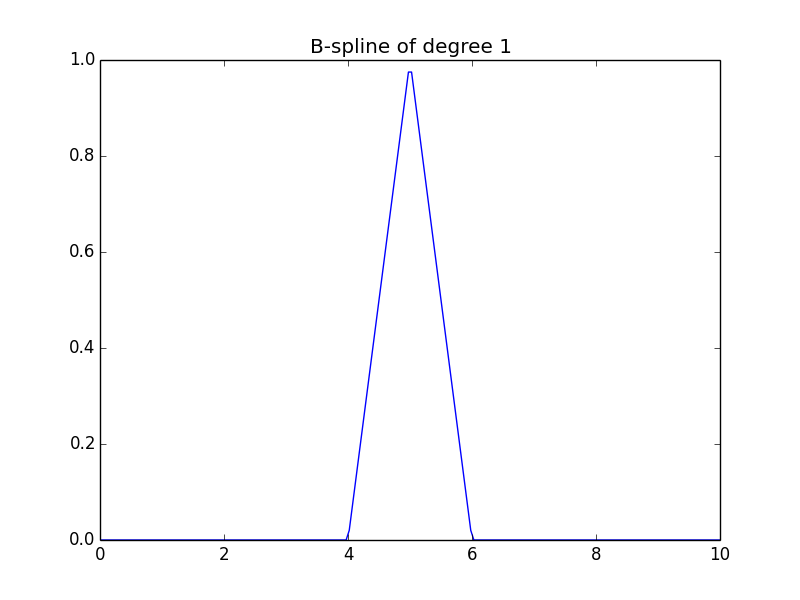
\includegraphics[width = 0.3\textwidth]{\figurespath/bsplines1.png}
		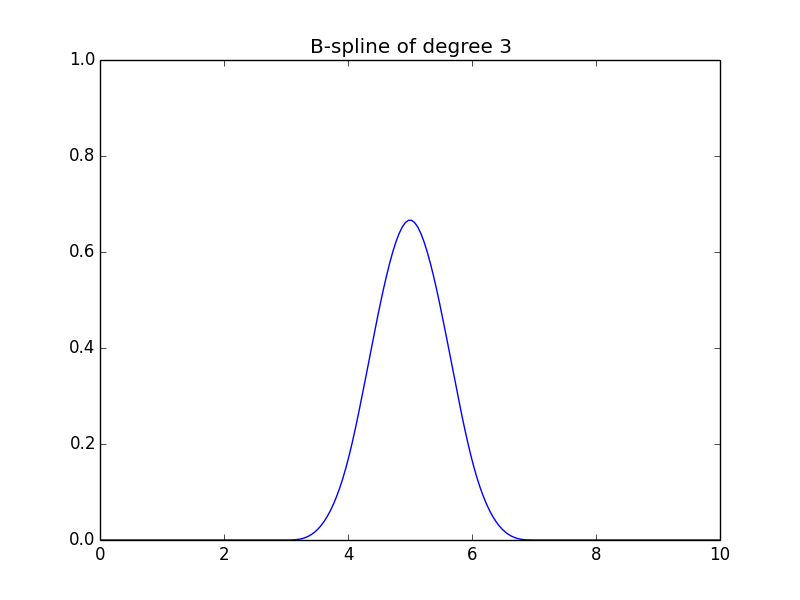
\includegraphics[width = 0.3\textwidth]{\figurespath/bsplines3.png}
		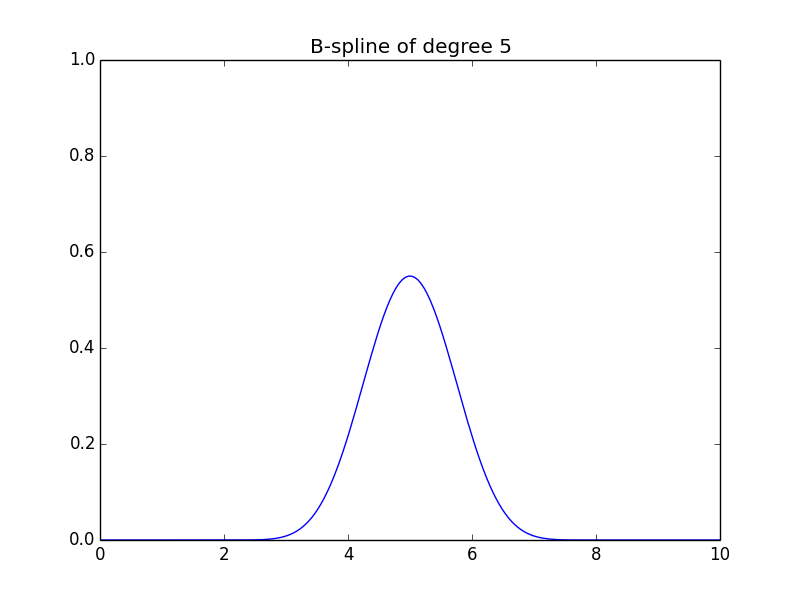
\includegraphics[width = 0.3\textwidth]{\figurespath/bsplines5.png}
	\end{center}

\end{frame}
% =================================


\end{document}

